\chapter{General Purpose Zero Knowledge Proofs}
In the voting schemes introduced in \cref{chap:votingschemes}, we employ \glspl{zkp} to ensure ballot validity.
Specifically, we use \glspl{gpzkp} over correct circuit execution to provide the ballot validity proofs.
Fundamentally, \glspl{gpzkp} allow us to prove any statement expressible inside an algebraic circuit.
Algebraic circuits are representations of algebraic functions.
We introduce \glspl{gpzkp} is a similar fashion to \cite{least_authority_moonmath_2024}.

\section{Algebraic Functions and Algebraic Circuts}
An algebraic circuit models an algebraic function $r$ that maps from a set of inputs to a set of outputs.
%An algebraic circuit represents a relation between a set of input signals and a set of output signals from a fixed field.
\begin{definition}[Algebraic Function]
    Let $(\mathbb{F}, +, \cdot)$ be a finite field.
    Let $m, n\in\mathbb{N}$ where $m$ is the number of input signals and $n$ is the number of output signals.
    Then, an algebraic function is defined as:
    \begin{align*}
        r:\mathbb{F}^m\to \mathbb{F}^n;\:(S_1^{in},\dots, S_{m}^{in})\mapsto (S_1^{out},\dots, S_n^{out})
    \end{align*}
    Here, the function needs to be expressible using the basic operations $+$ and $\cdot$ of $\mathbb{F}$.
\end{definition}

We can visualize the circuit for a function $r$ graphically as in \cref{fig:circuit:notation}.

%For every algebraic function $r$, there is a corresponding algebraic relation as defined in 

\begin{figure}[h]
    \centering
    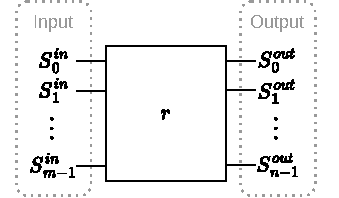
\includegraphics[scale=1]{graphics/circuits/Notation.pdf}
    \caption{Graphical representation of a circuit for the function $r:\mathbb{F}^m\to\mathbb{F}^n$.}
    \label{fig:circuit:notation}
\end{figure}

The basic operations $+$ and $\cdot$ are represented by the addition and multiplication gates in \cref{fig:circuit:addMul}.

\begin{figure}[h]
    \centering
    \begin{subfigure}{.48\textwidth}
        \centering
        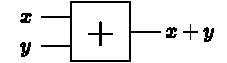
\includegraphics[scale=1]{graphics/circuits/Add.pdf}
    \end{subfigure}
    \hfill
    \begin{subfigure}{.48\textwidth}
        \centering
        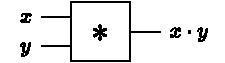
\includegraphics[scale=1]{graphics/circuits/Mul.pdf}
    \end{subfigure}
    \caption{Circuits for the basic field operation $+$ and $\cdot$ of $\mathbb{F}$.}
    \label{fig:circuit:addMul}
\end{figure}

% An example for an algebraic function is the $3$-factorization problem described in Example 118 of \cite{least_authority_moonmath_2024}:\\
% \begin{example}[$3$-factorization]
%     \label{exp:threeFac}
%     Let $\mathbb{F}=\mathbb{Z}_{13}$.
%     Then, the $3$-factorization problem is expressed by the algebraic function $r_{3\text{-}fac}$:
%     \begin{align*}
%         r_{3\text{-}fac}:\mathbb{Z}_{13}^3\to\mathbb{Z}_{13};\: (S_1^{in}, S_2^{in}, S_3^{in})\mapsto S_1^{out}=S_1^{in}\cdot S_2^{in}\cdot S_3^{in}
%     \end{align*}
%     $r_{3\text{-}fac}$ can therefore be represented by the circuit in \cref{fig:circuit:threeFac}.
% \end{example}
% 
% \begin{figure}[h]
%     \hfill
%     \begin{subfigure}{.48\textwidth}
%         \centering
%         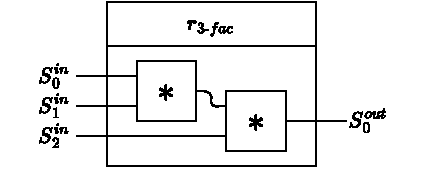
\includegraphics[scale=1]{graphics/circuits/ThreeFac_def}
%         \caption{Detailed Circuit.}
%         \label{fig:circuit:threeFacDef}
%     \end{subfigure}
%     \hfill
%     \begin{subfigure}{.48\textwidth}
%         \centering
%         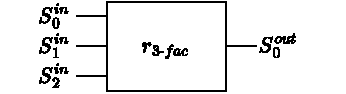
\includegraphics[scale=1]{graphics/circuits/ThreeFac_short.pdf}
%         \caption{Circuit Representation when used as a building block inside other circuits.}
%         \label{fig:circuit:threeFacShort}
%     \end{subfigure}
%     \hfill
%     \caption{Circuit for the $3$-factorization problem function $r_{3\text{-}fac}$.}
%     \label{fig:circuit:threeFac}
% \end{figure}

To see how algebraic functions can be used to indicate ballot validity, we consider our example from \cref{chap:votingschemes}.
Here, among other things, a voter needs to show that the ballot $b=(b_0,b_1,b_2)$ they chose is part of the choice space $C=\{(0,0,0),(1,0,0), (0,1,0), (0,0,1)\}$.
We can express this membership of the choice space by the function $r_{3\text{-}vot}$:
%\begin{example}[$3$-factorization]
%    \label{exp:threeFac}
    Let $(\mathbb{F},+,\cdot)$ be a finite field with $0,1\in\mathbb{F}$.
    Then, $r_{3\text{-}vot}$ is defined as:
    \begin{align*}
        r_{3\text{-}vot}:\mathbb{F}^3\to\mathbb{F}^4;\\
        (S_1^{in},S_2^{in}, S_3^{in})\mapsto (S_1^{out}, S_2^{out}, S_3^{out}, S_4^{out})
    \end{align*}
    Here, we can compute $S_1^{out}=r_{3\text{-}vot}(S_1^{in},S_2^{in}, S_3^{in})$ as in \cref{alg:threeVot}
    Note, that $r_{3\text{-}vot}(b_0,b_1,b_2)=(0,0,0,0)\Leftrightarrow (b_0,b_1,b_2)\in C$.

    $r_{3\text{-}vot}$ can be represented by the circuit in \cref{fig:circuit:exampleVoting}.
%\end{example}

\begin{Algorithmus}[h] %Use the environment only if you want to place the algorithm similar to graphics from TeX
    \caption{Function $r_{3\text{-}vot}$ used to check whether a ballot $b=(b_0,b_1,b_2)=(S_1^{in}, S_2^{in}, S_3^{in})$ is in the choice space $C=\{(0,0,0),(1,0,0),(0,1,0),(0,0,1)\}$. 
    $r_{3-\text{-}vot}$ returns $(0,0,0,0)$ if this is the case and something else otherwise.}
    \label{alg:threeVot}
    \begin{algorithmic}
    \Procedure{$r_{3-\text{-}vot}$}{$S_1^{in}, S_2^{in}, S_3^{in}$}
        \State $S_1^{out}:=(1-S_1^{in})\cdot S_1^{in}$
        \State $S_2^{out}:=(1-S_2^{in})\cdot S_2^{in}$
        \State $S_3^{out}:=(1-S_3^{in})\cdot S_3^{in}$ \Comment Determine whether the individual ballots are bits.
        \State $tmp:=S_1^{in}+S_2^{in}+S_3^{in}$
        \State $S_4^{out}:=(1-tmp)\cdot tmp$ \Comment Determine whether the sum of all ballots is a bit.
        \State \Return $(S_1^{out}, S_2^{out}, S_3^{out}, S_4^{out})$
    \EndProcedure
    \end{algorithmic}
\end{Algorithmus}

\begin{center}
\begin{figure}[h]
    
    \begin{subfigure}{.7\textwidth}
        \centering
        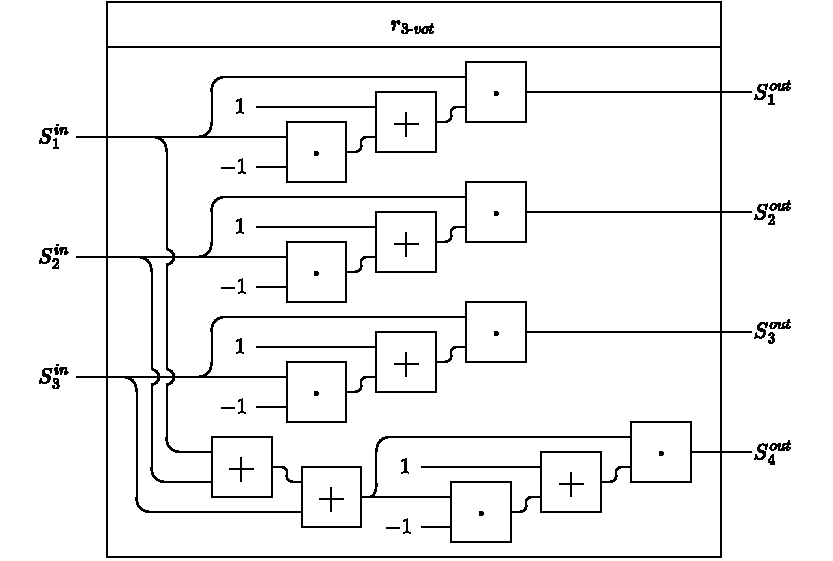
\includegraphics[scale=.8]{graphics/circuits/ExampleVoting_def}
        \caption{Detailed Circuit.}
        \label{fig:circuit:exampleVotingDef}
    \end{subfigure}
    \hfill
    \begin{subfigure}{.28\textwidth}
        \centering
        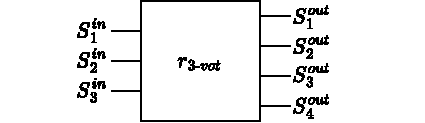
\includegraphics[scale=.8]{graphics/circuits/ExampleVoting_short.pdf}
        \caption{Circuit Representation when used as a building block inside other circuits.}
        \label{fig:circuit:exampleVotingShort}
    \end{subfigure}
    \hfill
    \caption{Circuit for the function $r_{3\text{-}vot}$, computing whether a ballot $b=(b_0,b_1,b_2)=(S_1^{in}, S_2^{in}, S_3^{in})$ is in the choice space $C=\{(0,0,0),(1,0,0),(0,1,0),(0,0,1)\}$.}
    \label{fig:circuit:exampleVoting}
\end{figure}
\end{center}


Now, we can assign arbitrary input and output values to the circuit for the function $r$.
If we then compute the algebraic function $r$ on the input values, this either yields the chosen output values or it yields something else.
If the computation results in the same output values as the ones chosen before, we say that the relation expressed by $r$ holds.
Furthermore, we can fix some of the input and output values of the circuit.
Then it is either possible to assign values to the rest of the signals such that the relation expressed by $r$ holds or it is not possible to do so.
We can formalize these ideas with the concept of relation satisfiability.

\begin{definition}[Relation Satisfiability]
    Let $(\mathbb{F}, +, \cdot )$ be a finite field.
    Let $r:\mathbb{F}^m\to \mathbb{F}^n$ be an algebraic function.
    
    Let $S=(S_1^{in}, \dots, S_{m}^{in}, S_1^{out},\dots, S_{n}^{out})$ be an assignment to $r$.
    Here:
    \begin{align*}
        \forall i\in\{1,\dots, m\}\forall j\in\{1,\dots, n\}:\:S_i^{in},S_j^{out}\in\mathbb{F}
    \end{align*}
    We say that $S$ satisfies the relation expressed by $r$, if and only if $r(S_1^{in},\dots, S_{m}^{in})=(S_1^{out},\dots, S_{n}^{out})$.
    We call the relation expressed by $r$ satisfiable if there exists an assignment $S$ such that $S$ satisfies the relation expressed by $r$.
    
    Let $I=(I_1^{in}, \dots, I_{m}^{in}, I_1^{out},\dots, I_{n}^{out})$ be a partial assignment to $f$.
    Here:
    \begin{align*}
        \forall i\in\{1,\dots, m\}\forall j\in\{1,\dots, n\}:\:I_i^{in},I_j^{out}\in\mathbb{F}\cup\{\bot\}  
    \end{align*}
    We call the relation expressed by $r$ satisfiable under $I$ if there is an assignment $S'=(S'^{in}_1, \dots, S'^{in}_{m}, S'^{out}_1,\dots, S'^{out}_{n})$ that satisfies the relation expressed by $r$, where:
    \begin{align*}
        \forall i\in\{1,\dots, m\}\forall j\in\{1,\dots, n\}:\\
        S'^{in}_i=I_{i}^{in} \:\text{ if }\: I_{i}^{in}\neq \bot\\
        S'^{in}_j=I_{j}^{out} \:\text{ if }\: I_{j}^{out}\neq \bot
    \end{align*}
\end{definition}

% For instance, the assignment $(5,2,4,1)$ satisfies $r_{3\text{-}fac}$ since $5\cdot 2\cdot 4=1$ in $\mathbb{Z}_{13}$.
% Therfore, $r_{3\text{-}fac}$ is satisfiable.
% However, the assignment $(1,0,3,7)$ does not satisfy $r_{3\text{-}fac}$ since $1\cdot 0\cdot 3=0\neq 7$ in $\mathbb{Z}_{13}$.
% Similarily, $r_{3\text{-}fac}$ is satisfiable under the partial assignment $(\bot, 2, 4, \bot)$ but not under the partial assignment $(0,\bot, \bot, 1)$.

For instance, the assignment $(0,0,1,0,0,0,0)$ satisfies the relation expressed by $r_{3\text{-}vot}$ since $(0,0,1)\in C$.
Therfore, the relation expressed by $r_{3\text{-}vot}$ is satisfiable.
However, the assignment $(1,1,0,0,0,0,0)$ does not satisfy the relation expressed by $r_{3\text{-}vot}$ since $tmp=1+1=2$, $(1-2)\cdot 2=-2$ and therefore, $r_{3\text{-}vot}(1,1,0)=(0,0,0,-2)\neq(0,0,0,0)$.
Similarily, the relation expressed by $r_{3\text{-}vot}$ is satisfiable under the partial assignment $(\bot, \bot, 1, 0,0,0,0)$ but not under the partial assignment $(2,\bot, \bot, 0,0,0,0)$.

\section{Rank-1 Constraint Systems}
\label{def:r1cs}
Fundamentally, \glspl{r1cs} are systems of equations of a specific format between a set of variables.

\begin{definition}[Rank-1 Constraint System]
    \label{def:r1cs}
    Let $(\mathbb{F},+,\cdot )$ be a field, let $n,k\in\mathbb{N}$.
    Let $a_j^i,b_j^i,c_j^i\in\mathbb{F}$ be constants from $\mathbb{F}$ for every index $i\in\{0,\dots, n\}$ and $j\in\{0,\dots, k\}$.
    Then, a \gls{r1cs} $R$ is defined as the following set of $k$ equations over the variables $S_1,\dots, S_n\in\mathbb{F}$:
    \begin{align*}
        \left(a_0^1+\sum\limits_{j=1}^n a_j^1\cdot S_j\right)\cdot \left(b_0^1+\sum\limits_{j=1}^n b_j^1\cdot S_j\right) \:&=\: c_0^1+\sum\limits_{j=1}^n c_j^1\cdot S_j\\
        &\vdots\\
        \left(a_0^k+\sum\limits_{j=1}^n a_j^k\cdot S_j\right)\cdot \left(b_0^k+\sum\limits_{j=1}^n b_j^k\cdot S_j\right) \:&=\: c_0^k+\sum\limits_{j=1}^n c_j^k\cdot S_j\\
    \end{align*}
    Hence, $n$ is the number of variables involved in the \gls{r1cs} and $k$ is the number of equations or constraints of the system.
\end{definition}

Note, that we can represent any algebraic function $r:\mathbb{F}^m\to \mathbb{F}^n$ and therefore also any algebraic circuit as a \gls{r1cs} $R_r$, since we require that $r$ can be expressed using just the basic field operations $+$ and $\cdot $ of $\mathbb{F}$.

% For instance, we can represent $r_{3\text{-}fac}$ as an \gls{r1cs} as follows:\\
% First, we need to rewrite the definition of $r_{3\text{-}fac}$ since each constraint of a \gls{r1cs} can have at most one multiplication $\cdot $.
% This process is also called flattening \cite{least_authority_moonmath_2024}.
% \begin{align*}
%     S_1^{in}\cdot S_2^{in}\cdot S_3^{in}=S_1^{out}\Leftrightarrow \begin{array}{l}
%         S_1^{in}\cdot S_2^{in}=S_1^{tmp}\\
%         S_1^{tmp}\cdot S_3^{in}=S_1^{out}
%     \end{array}
% \end{align*}
% Therefore, we have five variables and two constraints, and set $n=5$ and $k=2$ for the \gls{r1cs}.
% Furthermore, we set the variables for the \gls{r1cs} as follows:
% \begin{align*}
%     (S_1,S_2,S_3,S_4,S_5) = (S_1^{in}, S_2^{in}, S_3^{in}, S_1^{tmp}, S_1^{out})
% \end{align*}
% 
% Then, we need to choose the constants $a_i^j, b_i^j, c_i^j$ for $i\in\{0,\dots, 5\}, j\in\{1,2\}$ as follows:
% \begin{align*}
%     a_0^1=0 && a_1^1=1 && a_2^1=0 && a_3^1=0 && a_4^1=0 && a_5^1=0\\
%     b_0^1=0 && b_1^1=0 && b_2^1=1 && b_3^1=0 && b_4^1=0 && b_5^1=0\\
%     c_0^1=0 && c_1^1=0 && c_2^1=0 && c_3^1=0 && c_4^1=1 && c_5^1=0\\
%     &&&&&&&&&&\\
%     a_0^2=0 && a_1^2=0 && a_2^2=0 && a_3^2=0 && a_4^2=1 && a_5^2=0\\
%     b_0^2=0 && b_1^2=0 && b_2^2=0 && b_3^2=1 && b_4^2=0 && b_5^2=0\\
%     c_0^2=0 && c_1^2=0 && c_2^2=0 && c_3^2=0 && c_4^2=0 && c_5^2=1\\
% \end{align*}
% 
% Now, we can construct the equation system:
% {\setlength{\mathindent}{0pt}
% \begin{align*}
%     &\scriptstyle \left(a_0^1+a_1^1\cdot S_1+a_2^1\cdot S_2 + a_3^1\cdot S_3 + a_4^1\cdot S_4 + a_5^1\cdot S_5\right)\cdot \left(b_0^1+b_1^1\cdot S_1+b_2^1\cdot S_2 + b_3^1\cdot S_3 + b_4^1\cdot S_4 + b_5^1\cdot S_5\right) = \left(c_0^1+c_1^1\cdot S_1+c_2^1\cdot S_2 + c_3^1\cdot S_3 + c_4^1\cdot S_4 + c_5^1\cdot S_5\right)\\
%     &\scriptstyle \left(a_0^2+a_1^2\cdot S_1+a_2^2\cdot S_2 + a_3^2\cdot S_3 + a_4^2\cdot S_4 + a_5^2\cdot S_5\right)\cdot \left(b_0^2+b_1^2\cdot S_1+b_2^2\cdot S_2 + b_3^2\cdot S_3 + b_4^2\cdot S_4 + b_5^2\cdot S_5\right) = \left(c_0^2+c_1^2\cdot S_1+c_2^2\cdot S_2 + c_3^2\cdot S_3 + c_4^2\cdot S_4 + c_5^2\cdot S_5\right)\\
%     &\scriptstyle\Leftrightarrow \begin{array}{l}
%         \scriptstyle\left(0+1\cdot S_1^{in}+0\cdot S_2^{in} + 0\cdot S_3^{in} + 0\cdot S_1^{tmp} + 0\cdot S_1^{out}\right)\cdot \left(0+0\cdot S_1^{in}+1\cdot S_2^{in} + 0\cdot S_3^{in} + 0\cdot S_1^{tmp} + 0\cdot S_1^{out}\right) = \left(0+0\cdot S_1^{in}+0\cdot S_2^{in} + 0\cdot S_3^{in} + 1\cdot S_1^{tmp} + 0\cdot S_1^{out}\right)\\
%         \scriptstyle\left(0+0\cdot S_1^{in}+0\cdot S_2^{in} + 0\cdot S_3^{in} + 1\cdot S_1^{tmp} + 0\cdot S_1^{out}\right)\cdot \left(0+0\cdot S_1^{in}+0\cdot S_2^{in} + 1\cdot S_3^{in} + 0\cdot S_1^{tmp} + 0\cdot S_1^{out}\right) = \left(0+0\cdot S_1^{in}+0\cdot S_2^{in} + 0\cdot S_3^{in} + 0\cdot S_1^{tmp} + 1\cdot S_1^{out}\right)\\
%     \end{array}
%     &\\
%     &\scriptstyle\Leftrightarrow \begin{array}{l}
%         \scriptstyle S_1^{in}\cdot S_2^{in} = S_1^{tmp}\\
%         \scriptstyle S_1^{tmp}\cdot S_3^{in} = S_1^{out}\\
%     \end{array}
% \end{align*}
% }

% As we can see, this \gls{r1cs} does represent $f_{3\text{-}fac}$.

For instance, we can represent $r_{3\text{-}vot}$ as an \gls{r1cs} $R_{r_{3\text{-}vot}}$ as follows:\\
First, we need to rewrite the definition of $r_{3\text{-}vot}$ since each constraint of a \gls{r1cs} can have at most one multiplication $\cdot$.
This process is also called flattening \cite{least_authority_moonmath_2024}. We get:
\begin{align*}
    S_4^{out}=(1-S_1^{in}-S_2^{in}-S_3^{in})\cdot (S_1^{in}+S_2^{in}+S_3^{in})
\end{align*}
Together with the compuations for $S_1^{out}$, $S_2^{out}$ and $S_3^{out}$ which remain unchanged, we have seven variables and four constraints.
Therefore, we set $n=7$ and $k=7$ for the \gls{r1cs} and set the variables as follows:
\begin{align*}
    (S_1,S_2,S_3,S_4,S_5,S_6,S_7) = (S_1^{in}, S_2^{in}, S_3^{in}, S_1^{out}, S_2^{out}, S_3^{out}, S_4^{out})
\end{align*}

Then, we need to choose the constants $a_i^j, b_i^j, c_i^j$ for $i\in\{0,\dots, 7\}, j\in\{1,2,3,4\}$ as follows:
\begin{align*}
    \text{For } S_1^{out}:&&&&&&&&&&&&&&\\
    a_0^1=1 && a_1^1=-1 && a_2^1=0 && a_3^1=0 && a_4^1=0 && a_5^1=0 && a_6^1=0 && a_7^1=0\\
    b_0^1=0 && b_1^1=1 && b_2^1=0 && b_3^1=0 && b_4^1=0 && b_5^1=0 && b_6^1=0 && b_7^1=0\\
    c_0^1=0 && c_1^1=0 && c_2^1=0 && c_3^1=0 && c_4^1=1 && c_5^1=0 && c_6^1=0 && c_7^1=0\\
    &&&&&&&&&&&&&&\\
    \text{For } S_2^{out}:&&&&&&&&&&&&&&\\
    a_0^2=1 && a_1^2=0 && a_2^2=-1 && a_3^2=0 && a_4^2=0 && a_5^2=0 && a_6^2=0 && a_7^2=0\\
    b_0^2=0 && b_1^2=0 && b_2^2=1 && b_3^2=0 && b_4^2=0 && b_5^2=0 && b_6^2=0 && b_7^2=0\\
    c_0^2=0 && c_1^2=0 && c_2^2=0 && c_3^2=0 && c_4^2=0 && c_5^2=1 && c_6^2=0 && c_7^2=0\\
    &&&&&&&&&&&&&&\\
    \text{For } S_3^{out}:&&&&&&&&&&&&&&\\
    a_0^3=1 && a_1^3=0 && a_2^3=0 && a_3^3=-1 && a_4^3=0 && a_5^3=0 && a_6^3=0 && a_7^3=0\\
    b_0^3=0 && b_1^3=0 && b_2^3=0 && b_3^3=1 && b_4^3=0 && b_5^3=0 && b_6^3=0 && b_7^3=0\\
    c_0^3=0 && c_1^3=0 && c_2^3=0 && c_3^3=0 && c_4^3=0 && c_5^3=0 && c_6^3=1 && c_7^3=0\\
    &&&&&&&&&&&&&&\\
    \text{For } S_4^{out}:&&&&&&&&&&&&&&\\
    a_0^4=1 && a_1^4=-1 && a_2^4=-1 && a_3^4=-1 && a_4^4=0 && a_5^4=0 && a_6^4=0 && a_7^4=0\\
    b_0^4=0 && b_1^4=1 && b_2^4=1 && b_3^4=1 && b_4^4=0 && b_5^4=0 && b_6^4=0 && b_7^4=0\\
    c_0^4=0 && c_1^4=0 && c_2^4=0 && c_3^4=0 && c_4^4=0 && c_5^4=0 && c_6^4=0 && c_7^4=1\\
\end{align*}

Now, we can construct the equation system:
{\setlength{\mathindent}{0pt}
\begin{align*}
    &\scriptscriptstyle \left(a_0^1+a_1^1 S_1+a_2^1 S_2 + a_3^1 S_3 + a_4^1 S_4 + a_5^1 S_5 + a_6^1 S_6 + a_7^1 S_7\right)\cdot \left(b_0^1+b_1^1 S_1+b_2^1 S_2 + b_3^1 S_3 + b_4^1 S_4 + b_5^1 S_5 + b_6^1 S_6 + b_7^1 S_7\right) = \left(c_0^1+c_1^1 S_1+c_2^1 S_2 + c_3^1 S_3 + c_4^1 S_4 + c_5^1 S_5 + c_6^1 S_6 + c_7^1 S_7\right)\\
    &\scriptscriptstyle \left(a_0^2+a_1^2 S_1+a_2^2 S_2 + a_3^2 S_3 + a_4^2 S_4 + a_5^2 S_5 + a_6^2 S_6 + a_7^2 S_7\right)\cdot \left(b_0^2+b_1^2 S_1+b_2^2 S_2 + b_3^2 S_3 + b_4^2 S_4 + b_5^2 S_5 + b_6^2 S_6 + b_7^2 S_7\right) = \left(c_0^2+c_1^2 S_1+c_2^2 S_2 + c_3^2 S_3 + c_4^2 S_4 + c_5^2 S_5 + c_6^2 S_6 + c_7^2 S_7\right)\\
    &\scriptscriptstyle \left(a_0^3+a_1^3 S_1+a_2^3 S_2 + a_3^3 S_3 + a_4^3 S_4 + a_5^3 S_5 + a_6^3 S_6 + a_7^3 S_7\right)\cdot \left(b_0^3+b_1^3 S_1+b_2^3 S_2 + b_3^3 S_3 + b_4^3 S_4 + b_5^3 S_5 + b_6^3 S_6 + b_7^3 S_7\right) = \left(c_0^3+c_1^3 S_1+c_2^3 S_2 + c_3^3 S_3 + c_4^3 S_4 + c_5^3 S_5 + c_6^3 S_6 + c_7^3 S_7\right)\\
    &\scriptscriptstyle \left(a_0^4+a_1^4 S_1+a_2^4 S_2 + a_3^4 S_3 + a_4^4 S_4 + a_5^4 S_5 + a_6^4 S_6 + a_7^4 S_7\right)\cdot \left(b_0^4+b_1^4 S_1+b_2^4 S_2 + b_3^4 S_3 + b_4^4 S_4 + b_5^4 S_5 + b_6^4 S_6 + b_7^4 S_7\right) = \left(c_0^4+c_1^4 S_1+c_2^4 S_2 + c_3^4 S_3 + c_4^4 S_4 + c_5^4 S_5 + c_6^4 S_6 + c_7^4 S_7\right)\\
    &\scriptscriptstyle\Leftrightarrow \begin{array}{l}
        \scriptscriptstyle\left(1-S_1^{in}\right)\cdot \left(S_1^{in}\right) = \left(S_1^{out}\right)\\
        \scriptscriptstyle\left(1-S_2^{in}\right)\cdot \left(S_2^{in}\right) = \left(S_2^{out}\right)\\
        \scriptscriptstyle\left(1-S_3^{in}\right)\cdot \left(S_3^{in}\right) = \left(S_3^{out}\right)\\
        \scriptscriptstyle\left(1-S_1^{in}-S_2^{in}-S_3^{in}\right)\cdot \left(S_1^{in}+S_2^{in}+S_3^{in}\right) = \left(S_4^{out}\right)\\
    \end{array}
\end{align*}
}

As we can see, this \gls{r1cs} $R_{r_{3\text{-}vot}}$ does represent $r_{3\text{-}vot}$.

\section{Quadratic Arithmetic Programs}
To use \glspl{r1cs} in \glspl{gpzkp}, we need to transform them into another different representation, namely \glspl{qap}.
For every \gls{r1cs} $R$, there is a corresponding \gls{qap} $QAP(R)$.

\begin{definition}[Quadratic Arithmetic Program]
    \label{def:qap}
    Let $(\mathbb{F},+,\cdot )$ be a field, let $n,k\in\mathbb{N}$.
    Let $a_j^i,b_j^i,c_j^i\in\mathbb{F}$ be constants from $\mathbb{F}$ for every index $i\in\{0,\dots, n\}$ and $j\in\{0,\dots, k\}$.
    Let $R$ be the corresponding \gls{r1cs} as in \cref{def:r1cs}.
    Let $m_1,\dots, m_k$ be arbitrary, invertible and distinct elements of $\mathbb{F}$.
    Then, the \gls{qap} corresponding to the \gls{r1cs} $R$ is defined as follows:
    \begin{align*}
        QAP(R)=\left\{T\in\mathbb{F}[x],\left\{A_j, B_j, C_j\in \mathbb{F}[x]\right\}_{j=0}^{n}\right\}
    \end{align*}
    Here, $T, A_j, B_j, C_j$ are polynomials over $\mathbb{F}$ with:
    \begin{itemize}
        \item $T(x):=\prod\limits_{l=1}^k(x-m_l)$ is a polynomial of degree $k$.
        \item $A_j, B_j, C_j$ are polynomials of degree $k-1$ defined by:
        \begin{align*}
            \forall j\in\{0,\dots, n\}\forall i\in\{1,\dots, k\}: \:A_j(m_i)=a_j^{i},\:B_j(m_i)=b_j^{i},\: C_j(m_i)=c_j^{i}
        \end{align*}
    \end{itemize}
\end{definition}

We can construct $QAP(R)$ from $R$ by executing the follwoing steps:
\begin{enumerate}
    \item Choose $k$ distinct, invertible elements $m_1,\dots, m_k\in\mathbb{F}$, one for each constraint in $R$.
    \item Compute the target polynomial $T$ as in \cref{def:qap}.
    \item Use Lagrange's method of polynomial interpolation as described in section 3.3.4 of \cite{least_authority_moonmath_2024} to compute the polynomials $A_j, B_j$ and $C_j$ as in \cref{def:qap}.
    Here, we need to use the set $S_{A_j}:=\{(m_1,a_j^1),\dots, (m_k, a_j^k)\}$ as the (evaluation point, value)-pairs for the construction of $A_j$. 
    Analogously, we use $S_{B_j}:=\{(m_1,b_j^1),\dots, (m_k, b_j^k)\}$ and $S_{C_j}:=\{(m_1,c_j^1),\dots, (m_k, c_j^k)\}$ for the construction of $B_j$ and $C_j$.
\end{enumerate}

Once again, we use $r_{3\text{-}vot}$ and the corresponding \gls{r1cs} $R_{r_{3\text{-}vot}}$ as an example.
To construct the corresponding $QAP(R_{r_{3\text{-}vot}})$, we first need to choose the elements $m_1,m_2,m_3,m_4\in\mathbb{F}$.
In order to obtain a specific \gls{qap} at the end, we need to choose the field $\mathbb{F}$.
To keep things simple, we choose the finite field $\mathbb{F}=\mathbb{F}_{13}$.
Now we can follow the instructions outlined previously:
\begin{enumerate}
    \item Since $R_{r_{3\text{-}vot}}$ has four constraints, we choose the four elements from $\mathbb{F}_{13}$:
    \begin{align*}
        m_1=2,\:m_2=4,\:m_3=5,\:m_4=7
    \end{align*}
    \item Then, we get the followng target polynomial:
    \begin{align*}
        T(x) &= (x-m_1)(x-m_2)(x-m_3)(x-m_4)\\
        &= (x-2)(x-4)(x-5)(x-7)\\
        &= (x+11)(x+9)(x+8)(x+6)\\
        &= (x^2+7x+8)(x^2+x+9)\\
        &= x^4+x^3+9x^2+7x^3+7x^2+11x+8x^2+8x+7\\
        &= x^4+8x^3+11x^2+6x+7
    \end{align*}
    \item Now, we need to use Lagrange interpolation to compute the polynomials $A_j, B_j, C_j$ for $j\in\{1,2,3,4\}$.
    Here, we use:
    \begin{align*}
        &\text{For } m_1=2:&&&&&&&&&&&&&&\\
        &\scriptstyle \phantom{\text{For }}A_0(2)=1 &&\scriptstyle A_1(2)=-1 &&\scriptstyle  A_2(2)=0 &&\scriptstyle  A_3(2)=0 &&\scriptstyle  A_4(2)=0 &&\scriptstyle  A_5(2)=0 &&\scriptstyle  A_6(2)=0 &&\scriptstyle  A_7(2)=0\\
        &\scriptstyle \phantom{\text{For }}B_0(2)=0 &&\scriptstyle B_1(2)=1 && \scriptstyle B_2(2)=0 && \scriptstyle B_3(2)=0 && \scriptstyle B_4(2)=0 && \scriptstyle B_5(2)=0 && \scriptstyle B_6(2)=0 && \scriptstyle B_7(2)=0\\
        &\scriptstyle \phantom{\text{For }}C_0(2)=0 &&\scriptstyle C_1(2)=0 && \scriptstyle C_2(2)=0 && \scriptstyle C_3(2)=0 && \scriptstyle C_4(2)=1 && \scriptstyle C_5(2)=0 && \scriptstyle C_6(2)=0 && \scriptstyle C_7(2)=0\\
        &&&&&&&&&&&&&&&\\
        &\text{For } m_2=4:&&&&&&&&&&&&&&\\
        &\scriptstyle \phantom{\text{For }}A_0(4)=1 &&\scriptstyle A_1(4)=0 &&\scriptstyle A_2(4)=-1 &&\scriptstyle  A_3(4)=0 &&\scriptstyle  A_4(4)=0 &&\scriptstyle  A_5(4)=0 &&\scriptstyle  A_6(4)=0 &&\scriptstyle  A_7(4)=0\\
        &\scriptstyle \phantom{\text{For }}B_0(4)=0 &&\scriptstyle B_1(4)=0 &&\scriptstyle B_2(4)=1 && \scriptstyle B_3(4)=0 && \scriptstyle B_4(4)=0 && \scriptstyle B_5(4)=0 && \scriptstyle B_6(4)=0 && \scriptstyle B_7(4)=0\\
        &\scriptstyle \phantom{\text{For }}C_0(4)=0 &&\scriptstyle C_1(4)=0 &&\scriptstyle C_2(4)=0 && \scriptstyle C_3(4)=0 && \scriptstyle C_4(4)=0 && \scriptstyle C_5(4)=1 && \scriptstyle C_6(4)=0 && \scriptstyle C_7(4)=0\\
        &&&&&&&&&&&&&&&\\
        &\text{For } m_3=5:&&&&&&&&&&&&&&\\
        &\scriptstyle \phantom{\text{For }}A_0(5)=1 &&\scriptstyle A_1(5)=0 &&\scriptstyle A_2(5)=0 &&\scriptstyle A_3(5)=-1 &&\scriptstyle  A_4(5)=0 &&\scriptstyle  A_5(5)=0 &&\scriptstyle  A_6(5)=0 &&\scriptstyle  A_7(5)=0\\
        &\scriptstyle \phantom{\text{For }}B_0(5)=0 &&\scriptstyle B_1(5)=0 &&\scriptstyle B_2(5)=0 &&\scriptstyle B_3(5)=1 && \scriptstyle B_4(5)=0 && \scriptstyle B_5(5)=0 && \scriptstyle B_6(5)=0 && \scriptstyle B_7(5)=0\\
        &\scriptstyle \phantom{\text{For }}C_0(5)=0 &&\scriptstyle C_1(5)=0 &&\scriptstyle C_2(5)=0 &&\scriptstyle C_3(5)=0 && \scriptstyle C_4(5)=0 && \scriptstyle C_5(5)=0 && \scriptstyle C_6(5)=1 && \scriptstyle C_7(5)=0\\
        &&&&&&&&&&&&&&&\\
        &\text{For } m_4=7:&&&&&&&&&&&&&&\\
        &\scriptstyle \phantom{\text{For }}A_0(7)=1 &&\scriptstyle A_1(7)=-1 &&\scriptstyle A_2(7)=-1 &&\scriptstyle A_3(7)=-1&&\scriptstyle A_4(7)=0 &&\scriptstyle A_5(7)=0 &&\scriptstyle A_6(7)=0 &&\scriptstyle A_7(7)=0\\
        &\scriptstyle \phantom{\text{For }}B_0(7)=0 &&\scriptstyle B_1(7)=1 && \scriptstyle B_2(7)=1 && \scriptstyle B_3(7)=1 &&\scriptstyle B_4(7)=0 &&\scriptstyle B_5(7)=0 &&\scriptstyle B_6(7)=0 &&\scriptstyle B_7(7)=0\\
        &\scriptstyle \phantom{\text{For }}C_0(7)=0 &&\scriptstyle C_1(7)=0 && \scriptstyle C_2(7)=0 && \scriptstyle C_3(7)=0 &&\scriptstyle C_4(7)=0 &&\scriptstyle C_5(7)=0 &&\scriptstyle C_6(7)=0 &&\scriptstyle C_7(7)=1\\
    \end{align*}
    By Lagrange's interpolation we know that $A_4, A_5, A_6, A_7, B_0, B_4, B_5, B_6, B_7, C_0, C_1, C_2$ and $C_3$ are the zero polynomial since they are polynomials of degree $k-1=3$ and are $0$ on $4$ points.
    Using the process described in section 3.3.4 of \cite{least_authority_moonmath_2024} we can calculate the other polynomials.\\
    Let $P\in \{A,B,C\}$, $j\in \{0,\dots,7\}$. 
    Let $p$ be the lower case equivalent of $P$. 
    Then we can compute the polynomial $P_j$ with $S_{P_j}=\{(m_1,p_j^1), (m_2, p_j^2), (m_3, p_j^3), (m_4, p_j^4)\}$ as follows:
    \begin{align*}
        P_j(x) &= p_j^1\cdot\frac{x-m_2}{m_1-m_2}\cdot\frac{x-m_3}{m_1-m_3}\cdot\frac{x-m_4}{m_1-m_4} 
            + p_j^2\cdot \frac{x-m_1}{m_2-m_1}\cdot\frac{x-m_3}{m_2-m_3}\cdot\frac{x-m_4}{m_2-m_4}\\
            &\phantom{=} + p_j^3\cdot \frac{x-m_1}{m_3-m_1}\cdot\frac{x-m_2}{m_3-m_2}\cdot\frac{x-m_4}{m_3-m_4} 
            + p_j^4\cdot \frac{x-m_1}{m_4-m_1}\cdot\frac{x-m_2}{m_4-m_2}\cdot\frac{x-m_3}{m_4-m_3}\\
            &\\
            &=  p_j^1\cdot\frac{x-4}{2-4}\cdot\frac{x-5}{2-5}\cdot\frac{x-7}{2-7} 
            + p_j^2\cdot\frac{x-2}{4-2}\cdot\frac{x-5}{4-5}\cdot\frac{x-7}{4-7}\\
            &\phantom{=} + p_j^3\cdot\frac{x-2}{5-2}\cdot\frac{x-4}{5-4}\cdot\frac{x-7}{5-7} 
            + p_j^4\cdot\frac{x-2}{7-2}\cdot\frac{x-4}{7-4}\cdot\frac{x-5}{7-5}\\
            &\\
            &=p_j^1\cdot \frac{x^3+6x^2+4x^2+11x+7x+3}{(-2)\cdot (-3)\cdot (-5)} %(x^2-9x+7)\cdot(x-7)
            +p_j^2\cdot \frac{x^3+6x^2+6x^2+10x+10x+8}{2\cdot (-1)\cdot (-3)}\\ %(x^2-7x+10)\cdot (x-7)
            &\phantom{=} +p_j^3\cdot \frac{x^3+6x^2+7x^2+3x+8x+9}{3\cdot 1\cdot (-2)} %(x^2-6x+8)\cdot (x-7)
            + p_j^4\cdot \frac{x^3+8x^2+7x^2+4x+8x+12}{5\cdot 3\cdot 2}\\ %(x^2-6x+8)\cdot (x-5)
            &\\
            &=p_j^1\cdot \frac{x^3+10x^2+5x+3}{9}
            + p_j^2\cdot \frac{x^3+12x^2+7x+8}{6}\\
            &\phantom{=} +p_j^3\cdot \frac{x^3+11x+9}{7}
            +p_j^4\cdot \frac{x^3+2x^2+12x+12}{4}
    \end{align*}
    \begin{align*}
        \phantom{P_j(x)}&=p_j^1\cdot 3\cdot (x^3+10x^2+5x+3) &&\quad \text{Since } 9^{-1}=3\\
            &\phantom{=} + p_j^2\cdot 11\cdot(x^3+12x^2+7x+8) &&\quad \text{Since } 6^{-1}=11\\
            &\phantom{=} + p_j^3\cdot 2\cdot(x^3+11x+9) &&\quad \text{Since } 7^{-1}=2\\
            &\phantom{=} + p_j^4\cdot 10\cdot(x^3+2x^2+12x+12) &&\quad \text{Since } 4^{-1}=10
    \end{align*}
    \begin{align*}
        \phantom{P_j(x)}&=p_j^1\cdot (3x^3+4x^2+2x+9) + p_j^2\cdot (11x^3+2x^2+12x+10)\\
            &\phantom{=} + p_j^3\cdot (2x^3+9x+5) + p_j^4\cdot (10x^3+7x^2+3x+3)\\
            &\\
            \phantom{P_j(x)}&=(3p_j^1+11p_j^2+2p_j^3+10p_j^4)x^3 + (4p_j^1+2p_j^2+0p_j^3+7p_j^4)x^2\\
            &\phantom{=} + (2p_j^1+12p_j^2+9p_j^3+3p_j^4)x + (9p_j^1+10p_j^2+5p_j^3+3p_j^4)
    \end{align*}

    By instantiating $P$ and $j$ accordingly, we get:
    \begin{itemize}
        \item $A_0$ with $S_{A_0}=\{(m_1,a_0^1), (m_2, a_0^2), (m_3, a_0^3), (m_4, a_0^4)\}=\{(2,1), (4,1), (5,1), (7,1)\}$:
        {\setlength{\mathindent}{2pt}
        \begin{align*}
            A_0(x) &= (3a_0^1+11a_0^2+2a_0^3+10a_0^4)x^3 + (4a_0^1+2a_0^2+0a_0^3+7a_0^4)x^2\\
            &\phantom{=} + (2a_0^1+12a_0^2+9a_0^3+3a_0^4)x + (9a_0^1+10a_0^2+5a_0^3+3a_0^4)
            &\\
            &=(3+11+2+10)x^3 + (4+2+0+7)x^2 + (2+12+9+3)x + (9+10+5+3)\\
            &=1
        \end{align*}
        }
        \item $A_1$ with $S_{A_1}=\{(2,-1), (4,0), (5,0), (7,-1)\}$:
        {\setlength{\mathindent}{2pt}
        \begin{align*}
            A_1(x) &=(-3+0+0-10)x^3 + (-4+0+0-7)x^2 + (-2+0+0-3)x + (-9+0+0-3)\\
            &=2x^2 + 8x + 1
        \end{align*}
        }
        \item $A_2$ with $S_{A_2}=\{(2,0), (4,-1), (5,0), (7,-1)\}$:
        {\setlength{\mathindent}{2pt}
        \begin{align*}
            A_2(x) &=(0-11+0-10)x^3 + (0-2+0-7)x^2 + (0-12+0-3)x + (0-10+0-3)\\
            &=5x^3 + 4x^2 + 11x
        \end{align*}
        }
        \item $A_3$ with $S_{A_3}=\{(2,0), (4,0), (5,-1), (7,-1)\}$:
        {\setlength{\mathindent}{2pt}
        \begin{align*}
            A_3(x) &=(0+0-2-10)x^3 + (0+0+0-7)x^2 + (0+0-9-3)x + (0+0-5-3)\\
            &=x^3 + 6x^2 + x + 5
        \end{align*}
        }

        \item $B_1$ with $S_{B_1}=\{(2,1), (4,0), (5,0), (7,1)\}$:
        {\setlength{\mathindent}{2pt}
        \begin{align*}
            B_1(x) &=(3+0+0+10)x^3 + (4+0+0+7)x^2 + (2+0+0+3)x + (9+0+0+3)\\
            &=11x^2 + 5x + 12
        \end{align*}
        }
        \item $B_2$ with $S_{B_2}=\{(2,0), (4,1), (5,0), (7,1)\}$:
        {\setlength{\mathindent}{2pt}
        \begin{align*}
            B_2(x) &=(0+11+0+10)x^3 + (0+2+0+7)x^2 + (0+12+0+3)x + (0+10+0+3)\\
            &=8x^3 + 9x^2 + 2x
        \end{align*}
        }
        \item $B_3$ with $S_{B_3}=\{(2,0), (4,0), (5,1), (7,1)\}$:
        {\setlength{\mathindent}{2pt}
        \begin{align*}
            B_3(x) &=(0+0+2+10)x^3 + (0+0+0+7)x^2 + (0+0+9+3)x + (0+0+5+3)\\
            &=12x^3 + 7x^2 + 12x + 8
        \end{align*}
        }

        \item $C_4$ with $S_{C_4}=\{(2,1), (4,0), (5,0), (7,0)\}$:
        {\setlength{\mathindent}{2pt}
        \begin{align*}
            C_4(x) &=(3+0+0+0)x^3 + (4+0+0+0)x^2 + (2+0+0+0)x + (9+0+0+0)\\
            &=3x^3 + 4x^2 + 2x + 9
        \end{align*}
        }
        \item $C_5$ with $S_{C_5}=\{(2,0), (4,1), (5,0), (7,0)\}$:
        {\setlength{\mathindent}{2pt}
        \begin{align*}
            C_5(x) &=(0+11+0+0)x^3 + (0+2+0+0)x^2 + (0+12+0+0)x + (0+10+0+0)\\
            &=11x^3 + 2x^2 + 12x + 10
        \end{align*}
        }
        \item $C_6$ with $S_{C_6}=\{(2,0), (4,0), (5,1), (7,0)\}$:
        {\setlength{\mathindent}{2pt}
        \begin{align*}
            C_6(x) &=(0+0+2+0)x^3 + (0+0+0+0)x^2 + (0+0+9+0)x + (0+0+5+0)\\
            &=2x^3 + 9x + 5
        \end{align*}
        }
        \item $C_7$ with $S_{C_7}=\{(2,0), (4,0), (5,0), (7,1)\}$:
        {\setlength{\mathindent}{2pt}
        \begin{align*}
            C_7(x) &=(0+0+0+10)x^3 + (0+0+0+7)x^2 + (0+0+0+3)x + (0+0+0+3)\\
            &=10x^3 + 7x^2 + 3x + 3
        \end{align*}
        }
    \end{itemize}
\end{enumerate}

Putting everything together, we get $QAP(R_{r_{3\text{-}vot}})$ as follows (when using $\mathbb{F}_{13}$ as the base field):
\begin{align*}
    QAP(R_{r_{3\text{-}vot}}) &= \left\{T, \left\{A_0, B_0, C_0\right\}, \left\{A_1, B_1, C_1\right\}, \left\{A_2, B_2, C_2\right\}, \left\{A_3, B_3, C_3\right\},\right.\\
    &\phantom{=}\left.\left\{A_4, B_4, C_4\right\}, \left\{A_5, B_5, C_5\right\}, \left\{A_6, B_6, C_6\right\}, \left\{A_7, B_7, C_7\right\}\right\}
\end{align*}
\begin{align*}
    \phantom{QAP(R_{r_{3\text{-}vot}})}&= \Bigl\{x^4+8x^3+11x^2+6x+7,
\end{align*}
\begin{align*}
    \phantom{QAP(R_{r_{3\text{-}vot}})}&\phantom{=bl} \{1,&& 0,&& 0\}, &&\\
    &\phantom{=bl} \{2x^2 + 8x + 1,&& 11x^2 + 5x + 12,&& 0\},&&\\
    &\phantom{=bl} \{5x^3 + 4x^2 + 11x,&& 8x^3 + 9x^2 + 2x,&& 0\},&&\\
    &\phantom{=bl} \{x^3 + 6x^2 + x + 5,&& 12x^3 + 7x^2 + 12x + 8,&& 0\},&&\\
    &\phantom{=bl} \{0,&& 0,&& 3x^3 + 4x^2 + 2x + 9\},&&\\
    &\phantom{=bl} \{0,&& 0,&& 11x^3 + 2x^2 + 12x + 10\},&&\\
    &\phantom{=bl} \{0,&& 0,&& 2x^3 + 9x + 5\},&&\\
    &\phantom{=bl} \{0,&& 0,&& 10x^3 + 7x^2 + 3x + 3\}&&\Bigr\}\\
\end{align*}



\section{Groth16 SNARKs}

